\newpage
\section{Ταξινόμηση}
\subsection{Εισαγωγή στους ταξινομητές}
Σε αυτή την ενότητα θα αναλύσουμε τους αλγορίθμους
ταξινόμησης και θα δούμε τη χρήση τους. Για τους αλγορίθμους
αυτούς χωρίζουμε το σύνολο των δεδομένων μας σε δυο μέρη:
\begin{itemize}
    \item Δεδομένα εκπαίδευσης (\textlatin{training dataset})
    \item Δεδομένα επαλήθευσής (\textlatin{testing dataset})
\end{itemize}
Τα πρώτα τα χρησιμοποιούμε έτσι ώστε ο αλγόριθμος να βρει
κάποιο μοτίβο στα δεδομένα με το οποίο θα μπορεί να
κατατάσσει τα καινούρια δεδομένα που δέχεται σε κάποια
από τις υπάρχουσες κλάσεις. Αυτή είναι και η διαδικασία
εκπαίδευσης του μοντέλου. Αφού η εκπαίδευση τελειώσει τότε
θα χρησιμοποιήσουμε τα δεδομένα επαλήθευσής για να
επιβεβαιώσουμε την ορθή λειτουργία του μοντέλου.
Υπάρχουν τρεις βασικοί τύποι ταξινομητών:
\begin{itemize}
    \item Δυαδικοί (\textlatin{binary})
    \item Πολλαπλών κλάσεων (\textlatin{multy-class})
    \item Πολλαπλών ετικετών (\textlatin{multy-label})
\end{itemize}

Οι δυαδικοί ταξινομητές χρησιμοποιούνται όταν έχουμε μόνο
δύο κλάσεις στις οποίες θέλουμε να εντάξουμε τα δεδομένα,
ή όταν η απάντηση που θέλουμε να πάρουμε από το μοντέλο
είναι δυαδικής φύσης. Για παράδειγμα, ένα πρόβλημα δυαδικής
φύσης θα ήταν να προβλέψουμε εάν ένας ασθενής έχει ή δεν
έχει μια ασθένειά σύμφωνα με τις εξετάσεις του.

Οι ταξινομητές πολλαπλών κλάσεων από την άλλη είναι ικανοί
να αναγνωρίσουν περισσότερες από δύο κλάσεις και είναι πολύ
χρήσιμοι για την αναγνώρισή προτύπων. Συνεχίζοντας με το
προηγούμενο παράδειγμα θα θέλαμε χωρίσουμε τους ασθενείς
σύμφωνα με την κατάσταση τους σε:
\begin{itemize}
    \item υγιείς
    \item ήπια ασθένειά
    \item σοβαρή ασθένεια
\end{itemize}
Έτσι οι γιατροί θα μπορούν αν δράσουν ανάλογα.

Οι ταξινομητές πολλαπλών ετικετών δεν έχουν κάποια καινούρια
λογική αλλά εφαρμόζουν τις λογικές των προηγούμενων
προβλημάτων. Δηλαδή θα μπορούσαμε να θέλουμε να υλοποιήσουμε
ένα μοντέλο το οποίο να κάνει και τις δύο προηγούμενες
προβλέψεις που συζητήσαμε. Αυτά τα μοντέλα συνήθως δε
χρησιμοποιούν ξεχωριστούς αλγορίθμους αλλά συνδυάζουν
πολλούς ήδη γνωστούς αλγορίθμους για να φτάσουν στο
αποτέλεσμα.
\begin{figure}[H]
    \centering
    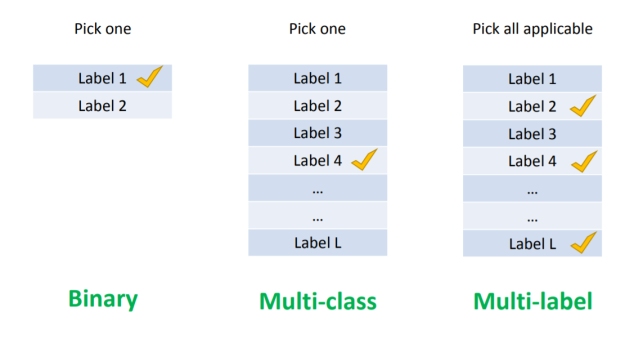
\includegraphics[width=0.5\textwidth]{images/typesOfClassifiers.png}
    \caption{Τύποι ταξινομητών}
\end{figure}

Στη συνέχεια θα αναλύσουμε τους διασημότερους αλγορίθμους
και τη χρήση τους. Οι αλγόριθμοι αυτοί είναι:
\begin{itemize}
    \item \textlatin{Naive Bayes}
    \item \textlatin{SVM (Support Vector Machine)}
    \item \textlatin{k-NN (k Nearest Neighbors)}
    \item \textlatin{Decision trees}
    \item \textlatin{SGD (Stochastic Gradient Descent)}
    \item \textlatin{Random Forest}
    \item Νευρωνικά Δίκτυα \textlatin{Neural Networks}
    \item \textlatin{LDA (Linear Discriminant Analysis)}
    \item \textlatin{QDA (Quadratic Discriminant Analysis)}
\end{itemize}
Για τις πληροφορίες αυτές συμβουλευτήκαμε αυτές τις
πηγές \cite{algo7, algo8, algo82}.
\subsection{\textlatin{Naive Bayes}}
Σύμφωνα με το παρακάτω άρθρο \cite{webb2010naive} ο αλγόριθμος \textlatin{Naive Bayes} είναι
ένας αλγόριθμος που κάνει την υπόθεση ότι τα χαρακτηριστικά είναι υπό όρους ανεξάρτητα της
δεδομένης κλάσης. Αυτή η υπόθεση στην πραγματικότητα δεν ισχύει αλλά ο αλγόριθμος πετυχαίνει
πολύ υψηλή ακρίβεια και ταυτόχρονα μεγάλη υπολογιστική απόδοση. Αυτός είναι και ο λόγος που
χρησιμοποιείται τόσο συχνά στην επιστήμη των δεδομένων. Τα πλεονεκτήματα του αλγορίθμου
είναι:
\begin{itemize}
    \item Η χρονική πολυπλοκότητα αυξάνεται γραμμικά με το πλήθος των δειγμάτων και των
    στοιχείων τους
    \item Χαμηλό \textlatin{variance} (η αλλαγή των δεδομένων δεν επηρεάζει πολύ το μοντέλο)
    \item Μπορούμε εύκολα να προσθέσουμε και άλλα δεδομένα και το μοντέλο θα συνεχίσει την
    εκπαίδευση χωρίς πρόβλημα
    \item Δεν είναι επιρρεπής στον θόρυβο
    \item Δεν επηρεάζεται από έλλειψη τιμών στα δεδομένα
\end{itemize}

Ο αλγόριθμος χρησιμοποιεί τον κανόνα του \textlatin{Bayes}:
$$P(y|X)=\frac{P(y)\times{P(X|y)}}{P(X)}$$
Ο παραπάνω τύπος θα μας δώσει την πιθανότητα ενός δείγματος με στοιχεία $X$ να ανήκει στην
κλάση $y$. Το $X$ είναι διάνυσμα με όλα τα στοιχεία του δείγματος μας. Στο παρακάτω
παράδειγμα το $X$ για το πρώτο δείγμα θα είναι $\langle40,85\rangle$ και η κλάση θα είναι
$y=0$. Σκοπός μας είναι όταν πάρουμε τα στοιχεία από έναν ασθενή να μπορούμε να προβλέψουμε
αν έχει διαβήτη. Θα πρέπει δηλαδή να υπολογίσουμε τις πιθανότητες

\begin{table}[H]
    \centering
    \begin{tabular}{|c|c|c|} \hline
        Γλυκόζη & Αρτηριακή πίεση & Διαβήτης \\ \hline
        40 & 85 & 0 \\ \hline
        40 & 92 & 0 \\ \hline
        45 & 63 & 1 \\ \hline
        45 & 80 & 0 \\ \hline
        40 & 73 & 1 \\ \hline
        45 & 82 & 0 \\ \hline
        40 & 85 & 0 \\ \hline
        30 & 63 & 1 \\ \hline
        65 & 65 & 1 \\ \hline
        45 & 82 & 0 \\ \hline
        35 & 73 & 1 \\ \hline
        45 & 90 & 0 \\ \hline
        50 & 68 & 1 \\ \hline
        40 & 93 & 0 \\ \hline
        35 & 80 & 1 \\ \hline
        50 & 70 & 1 \\ \hline
    \end{tabular}
\end{table}